\chapter{Experimental results}\label{ch:experiments}
%************************************************ 

In this chapter, we start by detailing in section \ref{sec:technologies} the choice of technologies in order to obtain experimental results. After that, these results will be discussed in order of application in sections \ref{sec:res_fs} (feature selection), \ref{sec:res_so} (structure optimization) and \ref{sec:res_lo} (learning optimization). By the end, we will have empirical evidence to point us in promising directions, which we will subsequently address when we talk about conclusions and future work.

\section{Software and hardware}\label{sec:technologies}

	\subsection{Software}

		The first decision to make is which programming language to use. \texttt{Python} is the choice for the following reasons:

		\begin{itemize}

			\item
			Previous experience with the language in web and machine learning applications.

			\item
			Popularity of the language, which is a good indicator of community support. According to the \textit{StackOverflow} 2018 Survey \footnote{\href{https://insights.stackoverflow.com/survey/2018/\#technology-programming-scripting-and-markup-languages}{\textit{StackOverflow} 2018 Survey: Most popular technologies}}, it is one of the most popular languages, and more so if we compare it with those commonly associated with machine learning in the last few years.

			\item
			Popularity of its machine learning and deep learning frameworks. Well-established frameworks include \texttt{Scikit-learn} \footnote{\href{https://github.com/scikit-learn/scikit-learn}{\texttt{Scikit-learn} GitHub repository}}, \\ \texttt{Caffe} \footnote{\href{https://github.com/BVLC/caffe}{\texttt{Caffe} GitHub repository}}, \texttt{TensorFlow} \footnote{\href{https://github.com/tensorflow/tensorflow}{\texttt{TensorFlow} GitHub repository}} and \texttt{Theano} \footnote{\href{https://github.com/Theano/Theano}{\texttt{Theano} GitHub repository}}. The last two of them also function as backends for the high-level neural networks API \texttt{Keras} \footnote{\href{https://github.com/keras-team/keras}{\texttt{Keras} GitHub repository}}. If we look at the number of stars in their \textit{GitHub} repositories, we can see that they are widely acknowledged by the community.

		\end{itemize}

\newpage

		The next step is choosing the tools to support our work. Since one of the goals of this project was to learn about optimization techniques, the genetic algorithm has been implemented from scratch, although there are alternatives like \texttt{DEAP} \footnote{\href{https://github.com/DEAP/deap}{\texttt{DEAP} GitHub repository}} if one wishes to avoid the additional development effort.

		Data operations become faster and easier with \texttt{Numpy} \footnote{\href{https://github.com/numpy/numpy}{\texttt{Numpy} GitHub repository}}. This will allow us to manage populations in genetic algorithms, as well as perform basic operations in a vectorized way whenever we need them. It is also fully compatible with the other libraries.

		Building machine learning models from scratch too is understandably out of the question. For this reason, we will rely on \texttt{Scikit-learn} for general machine learning algorithms and metrics, and on \texttt{Keras}---with its default \texttt{TensorFlow} backend---for neural networks.

		Lastly, many charts will be generated using \texttt{R} \footnote{\href{https://www.r-project.org/}{\texttt{R} Project website}}, which provides simple and powerful functionality for this task.

	\subsection{Hardware}

		We can make a distinction in this regard between the main development system, used for testing and debugging, and the dedicated servers for full-scale experimentation:

		\begin{itemize}

			\item
			Development system:

			\begin{itemize}

				\item
				Intel® Core™ i5-3470 CPU @ 3.20GHz, 8GB DDR3.
				\item
				NVIDIA GeForce® GTX 960, 2GB GDDR5.

			\end{itemize}

			\item
			First dedicated server:

			\begin{itemize}

				\item
				Intel® Xeon® E5-2620 v2 @ 2.10GHz, 32GB DDR3.
				\item
				NVIDIA Tesla® K20c, 5GB GDDR5.

			\end{itemize}

			\item
			Second dedicated server:

			\begin{itemize}

				\item
				Intel® Xeon® E5-2620 v4 @ 2.10GHz, 32GB DDR4.
				\item
				NVIDIA Tesla® K40m, 12GB GDDR5.

			\end{itemize}

			\item
			Third dedicated server:

			\begin{itemize}

				\item
				Two Intel® Xeon® E5-2620 v4 @ 2.10GHz, 32GB DDR4.
				\item
				NVIDIA Tesla® K40m, 12GB GDDR5.

			\end{itemize}

		\end{itemize}

\newpage

\section{Feature selection}\label{sec:res_fs}

	Determining the right configuration for the genetic algorithm---or rather, even one that is good enough---is no trivial task. Early experimentation seemed to point to a high crossover probability, but especially to a high mutation probability (ultimately set to 1). We will elaborate on that soon.

	Let us start by comparing three different crossover operators: \textit{Uniform}, \textit{Single-point} and \textit{Two-point}. We will work with a population of 300 individuals and 150 generations. We will set a 0.9 crossover probability after which a mutation will always ensue. A maximum of 50 active features will be allowed in each individual. The fitness criteria will take into account the Kappa value (for test accuracy) and a 5-fold cross-validation (for generalization assessment) measured for Logistic Regression.

	We will do an initial test run on each subject (104, 107 and 110). 

	Figure \ref{gfx:fs_crossover_kappa} displays the evolution of the mean Kappa error for all crossover operators in all three subjects.

    \begin{figure}[h]

        \begin{center}

        	\setlength{\fboxrule}{0pt}
            \fbox{
				\begin{varwidth}{\textwidth}
					\centering
					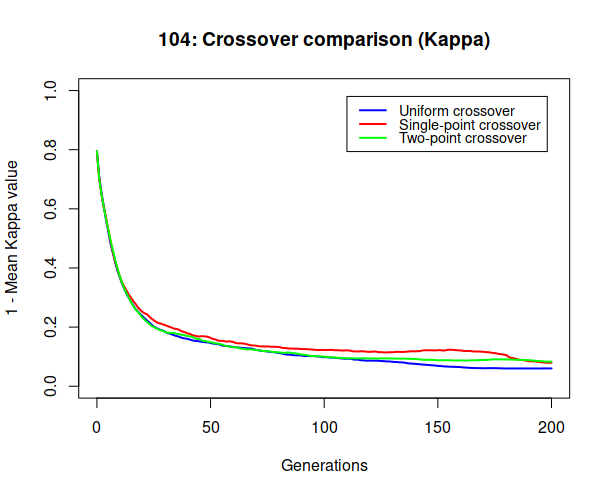
\includegraphics[width=0.45\textwidth]{gfx/FS_Crossover_Kappa_104.png}
				\end{varwidth}
			}
			\fbox{
				\begin{varwidth}{\textwidth}
					\centering
					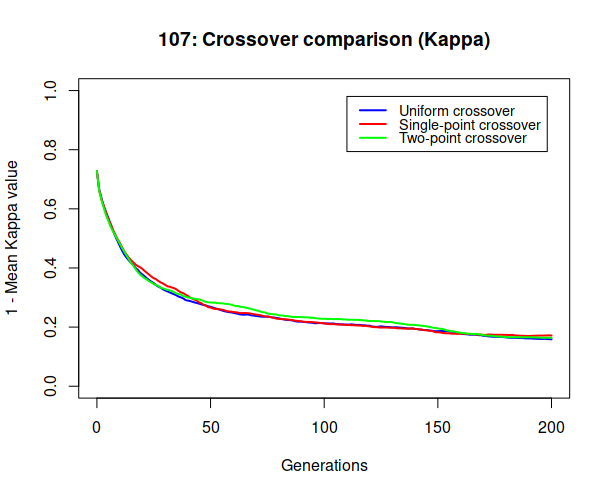
\includegraphics[width=0.45\textwidth]{gfx/FS_Crossover_Kappa_107.png}
				\end{varwidth}
			}
            \fbox{
				\begin{varwidth}{\textwidth}
					\centering
					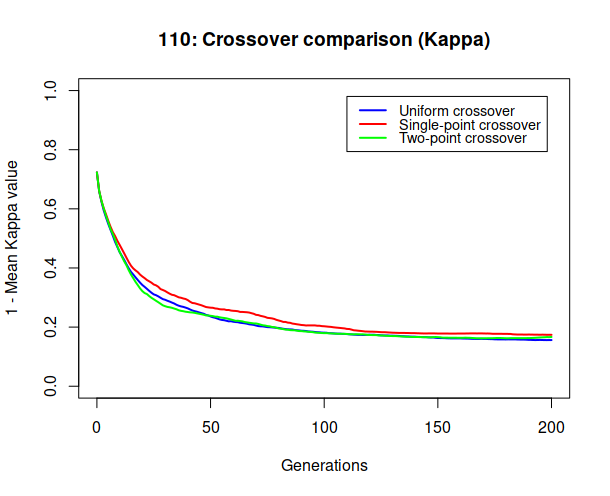
\includegraphics[width=0.45\textwidth]{gfx/FS_Crossover_Kappa_110.png}
				\end{varwidth}
			}

		\end{center}
		\caption[Kappa loss comparison for different crossovers]{Comparison of Kappa loss evolution over time with different crossover operators.}\label{gfx:fs_crossover_kappa}

	\end{figure}

	We can identify appreciable differences between the three curves: the blue one (uniform crossover) shows consistently better results than the other two, and the red one (single-point crossover) appears to be the worst.

\newpage

	Let us move on now to the same type of chart but with the cross-validation error (Figure \ref{gfx:fs_crossover_cv}). Again, the uniform crossover operator achieves the top performance across all individuals and the single-point crossover operator often lags behind.

	\begin{figure}[h]

        \begin{center}

        	\setlength{\fboxrule}{0pt}
            \fbox{
				\begin{varwidth}{\textwidth}
					\centering
					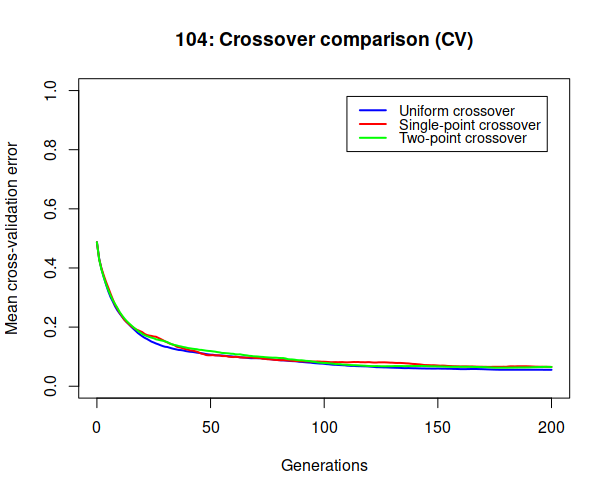
\includegraphics[width=0.45\textwidth]{gfx/FS_Crossover_CV_104.png}
				\end{varwidth}
			}
			\fbox{
				\begin{varwidth}{\textwidth}
					\centering
					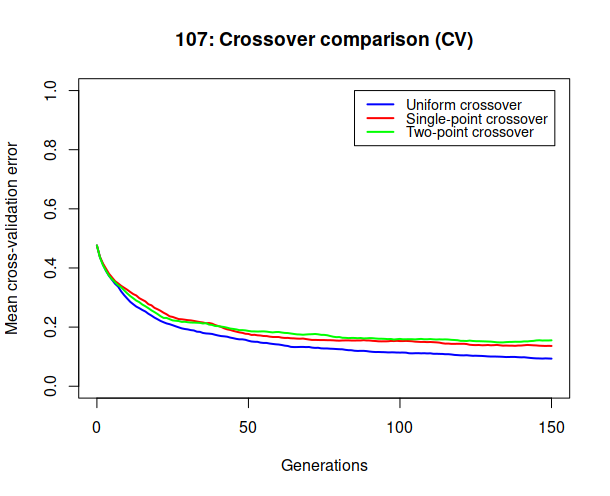
\includegraphics[width=0.45\textwidth]{gfx/FS_Crossover_CV_107.png}
				\end{varwidth}
			}
            \fbox{
				\begin{varwidth}{\textwidth}
					\centering
					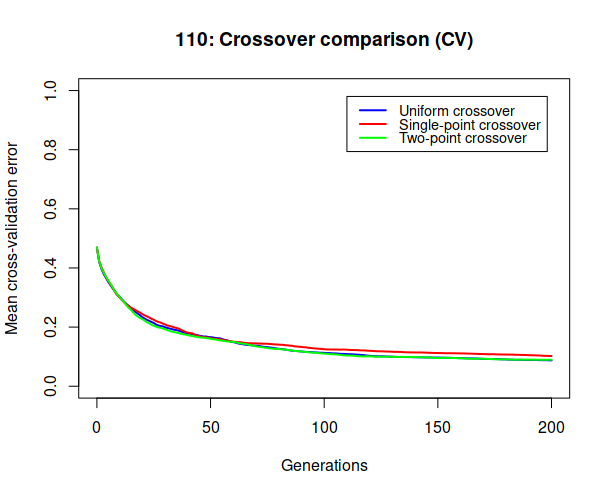
\includegraphics[width=0.45\textwidth]{gfx/FS_Crossover_CV_110.png}
				\end{varwidth}
			}

		\end{center}
		\caption[CV loss comparison for different crossovers]{Comparison of cross-validation loss evolution over time with different crossover operators.}\label{gfx:fs_crossover_cv}

	\end{figure}

	We seem to be spotting a trend that depends on the crossover operator. However, is it wise to extrapolate from only one test run? The answer is no: the running times allow us to repeat the experiment several times and find out whether their differences are statistically significant.

	As a compromise between quantity of samples and time expended, we will analyze 15 samples per crossover operator using their Kappa error values. Table \ref{table:crossover_kappa} shows the resulting values for all possible combinations:

	\vspace{0.3cm}

	\begin{table}[h]

        \centering
        \setlength\arrayrulewidth{0.8pt}

        \begin{tabular}{| >{\centering\arraybackslash}m{0.5in} | >{\centering\arraybackslash}m{1.1in} | >{\centering\arraybackslash}m{1.1in} | >{\centering\arraybackslash}m{1.1in} |}

            \hline
            \rowcolor{RoyalBlue}
            \textbf{Subject} & \textbf{Uniform} & \textbf{Single-point} & \textbf{Two-point} \\
            \hline
            \textbf{104} & $0.06534 \pm 0.0074$ & $0.08619 \pm 0.0102$ & $0.07941 \pm 0.0119$ \\
            \hline
            \textbf{107} & $0.15202 \pm 0.0132$ & $0.18004 \pm 0.0137$ & $0.17725 \pm 0.0150$ \\
            \hline
            \textbf{110} & $0.14829 \pm 0.0138$ & $0.17131 \pm 0.0158$ & $0.16569 \pm 0.0187$ \\
            \hline

        \end{tabular}

        \caption{Comparison of average Kappa error values for the three subjects and the three crossover operators.}\label{table:crossover_kappa}

    \end{table}

    The average performance of each operator seems to be what we expected. Additionally, the uniform crossover appears to produce slightly more stable results, judging from the standard deviation. Next, and not making assumptions about normality, we will perform a \textit{Kruskal-Wallis} test to see if their differences are worth considering. The \textit{p-values} are displayed in Tables \ref{table:crossover_kruskal_104}, \ref{table:crossover_kruskal_107} and \ref{table:crossover_kruskal_110}, with values below $0.05$ representing meaningful differences ($95\%$ confidence interval).

	\begin{table}[h]

        \centering
        \setlength\arrayrulewidth{0.8pt}

        \begin{tabular}{| >{\centering\arraybackslash}m{0.9in} | >{\centering\arraybackslash}m{0.9in} | >{\centering\arraybackslash}m{0.9in} |}

            \hline
            \rowcolor{RoyalBlue}
            \textbf{104} & \textbf{Single-point} & \textbf{Two-point} \\
            \hline
            \cellcolor{RoyalBlue}\textbf{Uniform} & $p = 0.000027$ & $p = 0.000835$ \\
            \hline
            \cellcolor{RoyalBlue}\textbf{Single-point} & \cellcolor{lightgray} & \textcolor{red}{$p = 0.056282$} \\
            \hline

        \end{tabular}

        \caption{Comparison of p-values for the crossover operators (subject 104).}\label{table:crossover_kruskal_104}

    \end{table}

    \begin{table}[h]

        \centering
        \setlength\arrayrulewidth{0.8pt}

        \begin{tabular}{| >{\centering\arraybackslash}m{0.9in} | >{\centering\arraybackslash}m{0.9in} | >{\centering\arraybackslash}m{0.9in} |}

            \hline
            \rowcolor{RoyalBlue}
            \textbf{107} & \textbf{Single-point} & \textbf{Two-point} \\
            \hline
            \cellcolor{RoyalBlue}\textbf{Uniform} & $p = 0.000023$ & $p = 0.000104$ \\
            \hline
            \cellcolor{RoyalBlue}\textbf{Single-point} & \cellcolor{lightgray} & \textcolor{red}{$p = 0.678133$} \\
            \hline

        \end{tabular}

        \caption{Comparison of p-values for the crossover operators (subject 107).}\label{table:crossover_kruskal_107}

    \end{table}

    \begin{table}[h]

        \centering
        \setlength\arrayrulewidth{0.8pt}

        \begin{tabular}{| >{\centering\arraybackslash}m{0.9in} | >{\centering\arraybackslash}m{0.9in} | >{\centering\arraybackslash}m{0.9in} |}

            \hline
            \rowcolor{RoyalBlue}
            \textbf{110} & \textbf{Single-point} & \textbf{Two-point} \\
            \hline
            \cellcolor{RoyalBlue}\textbf{Uniform} & $p = 0.000454$ & $p = 0.006561$ \\
            \hline
            \cellcolor{RoyalBlue}\textbf{Single-point} & \cellcolor{lightgray} & \textcolor{red}{$p = 0.299489$} \\
            \hline

        \end{tabular}

        \caption{Comparison of p-values for the crossover operators (subject 110).}\label{table:crossover_kruskal_110}

    \end{table}

    As we can see, the single-point and two-point crossovers show no statistically significant differences in their recorded results.

    The computational impact of either operator is negligible against the much more intensive fitness evaluations, so there is no reason not to consider the uniform crossover as our pick from now on. The last thing to do before moving on is attempt to explain why this happens. 

    On one hand, $n$-point crossovers merge large blocks from both parents; this leads to a not-so-optimal information transfer when trying to pick a handful of features from a pool of 3600.

    On the other hand, the uniform crossover is often said to be very disruptive, due to randomly choosing elements for which the parents do not agree. However, when only a small portion $k$ of features is active at a time, the disruption is at most $2k$ elements (the rest are inactive features); on top of that, features in which both parents agree are always kept. This makes the uniform crossover excel at \textit{exploitation} while also helping in \textit{exploration}. Together with frequent mutations, this is probably the key of the performance gain of the algorithm.

    Another aspect to look into is the effect of population sizes and number of generations. Bigger populations should introduce greater exploration possibilities, while more generations should allow the genetic algorithm to converge to even better solutions. Nevertheless, an increase in these parameters has a direct influence in computation times, so we will have to check if the improvement is worth the effort.

    We were working with a population size of 300 individuals and a number of generations equal to 150. The first alternative we propose is a tradeoff between a bigger population and less generations: 500 and 100. The second alternative is an increase in both: 800 individuals and 200 generations. Like we did before, we will start by observing what happens in a single run. In Figure \ref{gfx:fs_popgen_kappa} we can take a look at the behavior of the genetic algorithm in terms of Kappa loss.

    \vspace{0.3cm}

    \begin{figure}[h]

        \begin{center}

        	\setlength{\fboxrule}{0pt}
            \fbox{
				\begin{varwidth}{\textwidth}
					\centering
					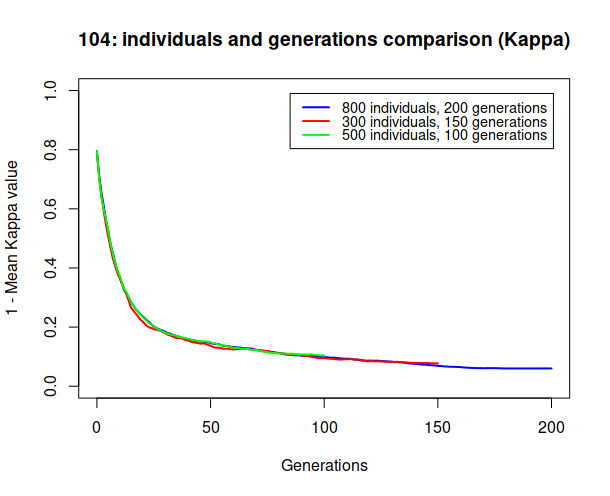
\includegraphics[width=0.45\textwidth]{gfx/FS_IndGens_Kappa_104.png}
				\end{varwidth}
			}
			\fbox{
				\begin{varwidth}{\textwidth}
					\centering
					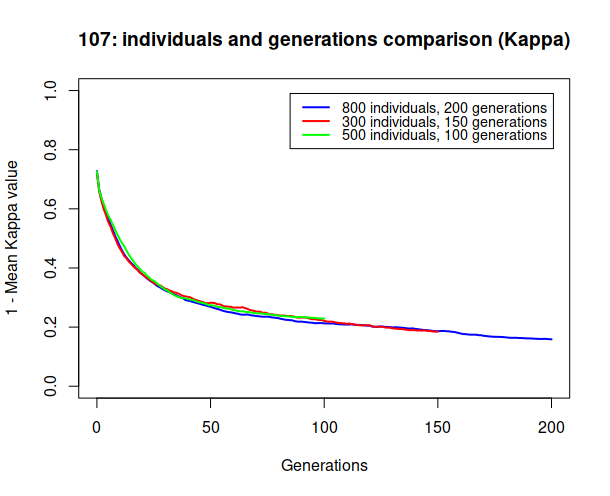
\includegraphics[width=0.45\textwidth]{gfx/FS_IndGens_Kappa_107.png}
				\end{varwidth}
			}
            \fbox{
				\begin{varwidth}{\textwidth}
					\centering
					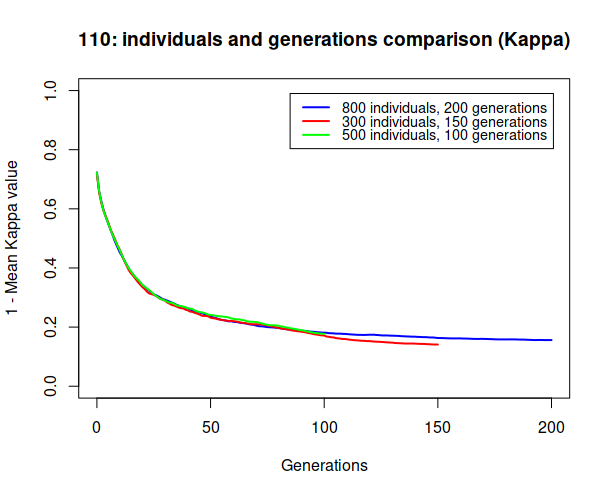
\includegraphics[width=0.45\textwidth]{gfx/FS_IndGens_Kappa_110.png}
				\end{varwidth}
			}

		\end{center}
		\caption[Kappa loss comparison for different populations and generations]{Comparison of Kappa loss evolution over time with different configurations of population and generations.}\label{gfx:fs_popgen_kappa}

	\end{figure}

	There is one definite conclusion we can draw: the number of generations is preventing the emergence of better individuals. The curves follow similar paths until they are progressively stopped by the generation limit. If we take a look at Figure \ref{gfx:fs_popgen_cv}, the same phenomenon is taking place for cross-validation loss, which does not surprise us.

\newpage

	\begin{figure}[bth]

        \begin{center}

        	\setlength{\fboxrule}{0pt}
            \fbox{
				\begin{varwidth}{\textwidth}
					\centering
					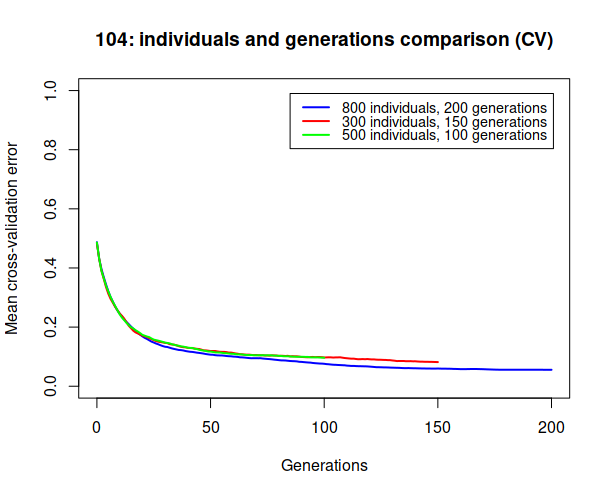
\includegraphics[width=0.45\textwidth]{gfx/FS_IndGens_CV_104.png}
				\end{varwidth}
			}
			\fbox{
				\begin{varwidth}{\textwidth}
					\centering
					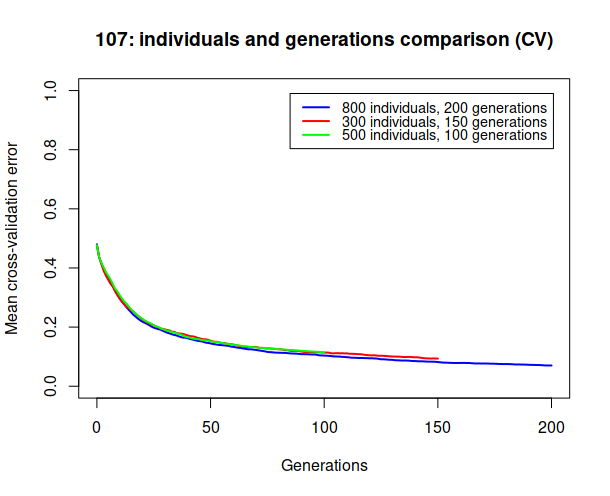
\includegraphics[width=0.45\textwidth]{gfx/FS_IndGens_CV_107.png}
				\end{varwidth}
			}
            \fbox{
				\begin{varwidth}{\textwidth}
					\centering
					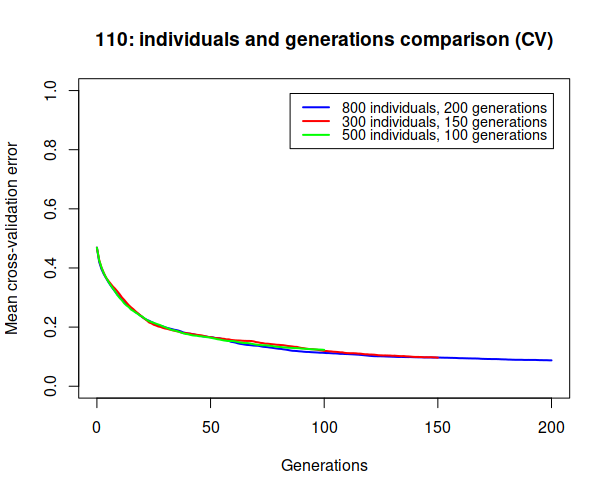
\includegraphics[width=0.45\textwidth]{gfx/FS_IndGens_CV_110.png}
				\end{varwidth}
			}

		\end{center}
		\caption[Cross-validation loss comparison for different populations and generations]{Comparison of cross-validation loss evolution over time with different configurations of population and generations.}\label{gfx:fs_popgen_cv}

	\end{figure}

	It is clear that we need a relevant analysis like that of crossover operators. We will keep the number of individuals intact to grant more diversity, but we have to confirm the importance of extending the evolutionary process. For all this, another 15 algorithm runs for each alternative will be used to make statistical claims.

	First, let us put the average performances alongside one another in Table \ref{table:popgen_kappa}:

	\vspace{0.3cm}

	\begin{table}[h]

        \centering
        \setlength\arrayrulewidth{0.8pt}

        \begin{tabular}{| >{\centering\arraybackslash}m{0.5in} | >{\centering\arraybackslash}m{1.1in} | >{\centering\arraybackslash}m{1.1in} | >{\centering\arraybackslash}m{1.1in} |}

            \hline
            \rowcolor{RoyalBlue}
            \textbf{Subject} & \textbf{300-150} & \textbf{500-100} & \textbf{800-200} \\
            \hline
            \textbf{104} & $0.06534 \pm 0.0074$ & $0.06310 \pm 0.0077$ & $0.05127 \pm 0.0067$ \\
            \hline
            \textbf{107} & $0.15202 \pm 0.0132$ & $0.16830 \pm 0.0145$ & $0.12122 \pm 0.0126$ \\
            \hline
            \textbf{110} & $0.14829 \pm 0.0138$ & $0.15448 \pm 0.0069$ & $0.13369 \pm 0.0083$ \\
            \hline

        \end{tabular}

        \caption{Comparison of average Kappa error values for the three subjects and the three configurations.}\label{table:popgen_kappa}

    \end{table}

    We see that taking the population size up to 800 and the generations up to 200 yields finer average results. It is also noticeable that a bigger population appears to matter less when the number of generations is not accordingly increased.

\newpage

    Tables \ref{table:popgen_kruskal_104}, \ref{table:popgen_kruskal_107} and \ref{table:popgen_kruskal_110} show the Kruskal-Wallis p-values for every pair of combinations. Again, we work with a $95\%$ confidence interval, which means that values below $0.05$ point to statistically significant differences.

    \vspace{0.3cm}

    \begin{table}[h]

        \centering
        \setlength\arrayrulewidth{0.8pt}

        \begin{tabular}{| >{\centering\arraybackslash}m{0.9in} | >{\centering\arraybackslash}m{0.9in} | >{\centering\arraybackslash}m{0.9in} |}

            \hline
            \rowcolor{RoyalBlue}
            \textbf{104} & \textbf{300-150} & \textbf{500-100} \\
            \hline
            \cellcolor{RoyalBlue}\textbf{800-200} & $p = 0.000144$ & $p = 0.000301$ \\
            \hline
            \cellcolor{RoyalBlue}\textbf{300-150} & \cellcolor{lightgray} & \textcolor{red}{$p = 0.884484$} \\
            \hline

        \end{tabular}

        \caption{Comparison of p-values for the evolutionary configurations (subject 104).}\label{table:popgen_kruskal_104}

    \end{table}

    \begin{table}[h]

        \centering
        \setlength\arrayrulewidth{0.8pt}

        \begin{tabular}{| >{\centering\arraybackslash}m{0.9in} | >{\centering\arraybackslash}m{0.9in} | >{\centering\arraybackslash}m{0.9in} |}

        	\hline
            \rowcolor{RoyalBlue}
            \textbf{107} & \textbf{300-150} & \textbf{500-100} \\
            \hline
            \cellcolor{RoyalBlue}\textbf{800-200} & $p = 0.000016$ & $p = 0.000005$ \\
            \hline
            \cellcolor{RoyalBlue}\textbf{300-150} & \cellcolor{lightgray} & $p = 0.002441$ \\
            \hline

        \end{tabular}

        \caption{Comparison of p-values for the evolutionary configurations (subject 107).}\label{table:popgen_kruskal_107}

    \end{table}

    \begin{table}[h]

        \centering
        \setlength\arrayrulewidth{0.8pt}

        \begin{tabular}{| >{\centering\arraybackslash}m{0.9in} |  >{\centering\arraybackslash}m{0.9in} | >{\centering\arraybackslash}m{0.9in} |}

            \hline
            \rowcolor{RoyalBlue}
            \textbf{110} & \textbf{300-150} & \textbf{500-100} \\
            \hline
            \cellcolor{RoyalBlue}\textbf{800-200} & $p = 0.003392$ & $p = 0.000005$ \\
            \hline
            \cellcolor{RoyalBlue}\textbf{300-150} & \cellcolor{lightgray} & $p = 0.034037$ \\
            \hline

        \end{tabular}

        \caption{Comparison of p-values for the evolutionary configurations (subject 110).}\label{table:popgen_kruskal_110}

    \end{table}

    The first thing we notice is that the combination 800-200 is consistently different from the other two. The differences between 300-150 and 500-100 are not so clear at times (see individual 104), but we could say that in a general case the approach with more generations can arrive at better solutions.

    We find ourselves in a quandary between prioritizing computation times or results. The running times are certainly higher with 800-200, but they are still under an hour for a single subject, which means we can do a lot in a full day. On the side of quality, an improvement of just a few percentage points at this level can be invaluable. Given all this, we will keep the 800-200 configuration and make it our baseline for our forthcoming comparisons against neural networks.

    Another topic to cover is the choice of fitness metrics. In particular, we can foresee that a substantial number of features will lag the already slow training in neural networks. One way to solve this could involve adding a third fitness function to favor individuals with fewer features. Let us proceed to briefly evaluate this possibility.

    We will use a straightforward simplicity measure that returns the number of active features of an individual. The goal of the algorithm will be, like with the other two, to minimize it. Sample experiments with and without this simplicity measure can be observed in Figure \ref{gfx:fs_simplicity_kappa}.

    \vspace{0.3cm}

    \begin{figure}[bth]

        \begin{center}

        	\setlength{\fboxrule}{0pt}
            \fbox{
				\begin{varwidth}{\textwidth}
					\centering
					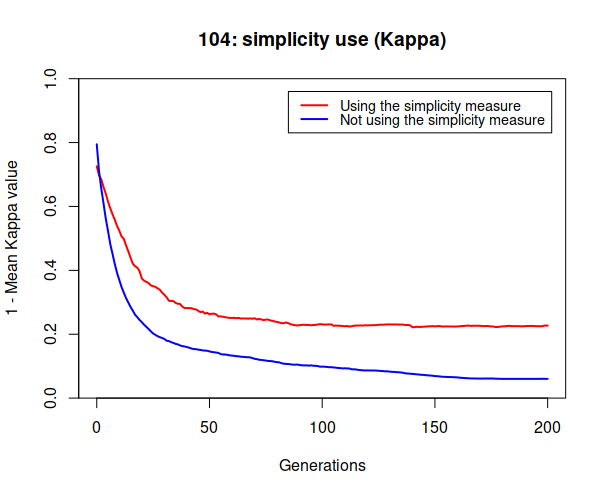
\includegraphics[width=0.45\textwidth]{gfx/FS_Simplicity_Kappa_104.png}
				\end{varwidth}
			}
			\fbox{
				\begin{varwidth}{\textwidth}
					\centering
					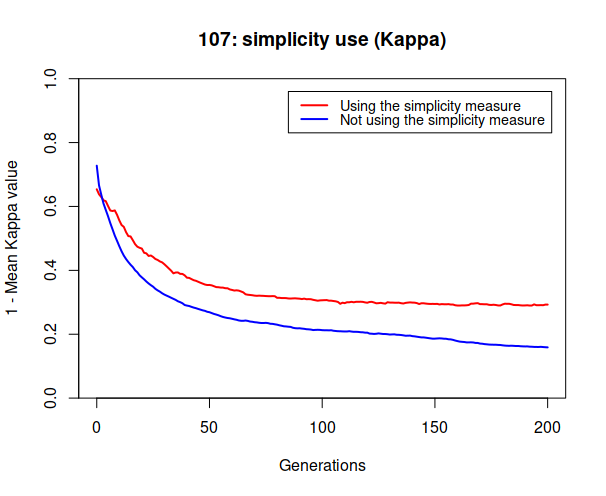
\includegraphics[width=0.45\textwidth]{gfx/FS_Simplicity_Kappa_107.png}
				\end{varwidth}
			}
            \fbox{
				\begin{varwidth}{\textwidth}
					\centering
					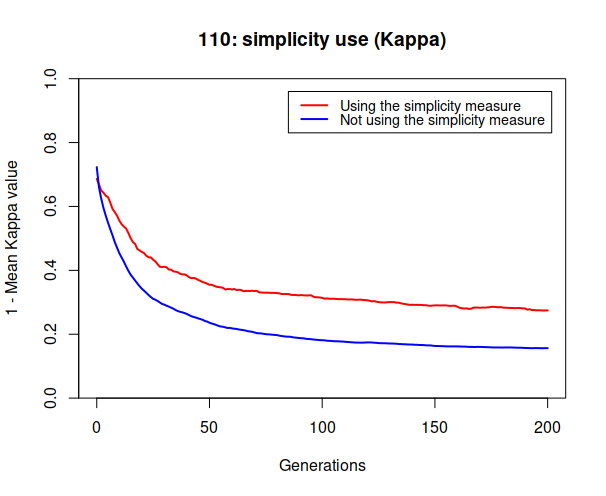
\includegraphics[width=0.45\textwidth]{gfx/FS_Simplicity_Kappa_110.png}
				\end{varwidth}
			}

		\end{center}
		\caption[Kappa loss comparison with and without simplicity]{Comparison of Kappa loss evolution over time with and without the simplicity measure. A similar phenomenon occurs with the cross-validation loss.}\label{gfx:fs_simplicity_kappa}

	\end{figure}

	The reported difference in performance is enormous. There is no need to do any statistical tests to realize that it will keep happening. The explanation is as easy as it gets: the simplicity measure hinders the progress of the other two criteria to the point of ultimately stalling it. In fact, for all we know there might be individuals with just one feature and abysmal accuracy in the first Pareto front.

	In order not to twist the original logic of the algorithm, we will just use the feature cap as a means to keep the number of features under control---more research could be done about where the optimal cap lies. The other two fitness measures will still be used, since they provide valuable assessment about accuracy on unseen data and generalization capability.

\newpage

	To wrap up this section, the last improvement we will introduce is the choice of models for the fitness functions. One could argue that introducing a better model would only confirm that the model is more suitable for the problem and not that it can find better features; however, since it is not possible to formally prove or disprove it, we will give it a go.

	This time, we will be measuring Logistic Regression against \ac{SVM}. Figure \ref{gfx:fs_models_kappa} shows the Kappa loss of a tentative run just to know if the comparison made any sense in the first place.

	\vspace{0.3cm}

    \begin{figure}[bth]

        \begin{center}

        	\setlength{\fboxrule}{0pt}
            \fbox{
				\begin{varwidth}{\textwidth}
					\centering
					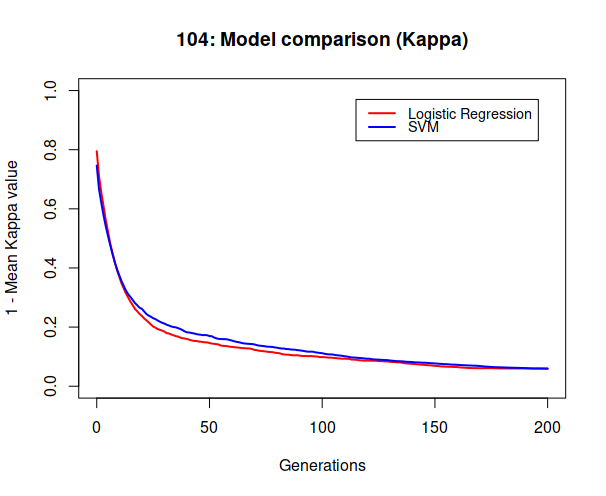
\includegraphics[width=0.45\textwidth]{gfx/FS_ModelComparison_Kappa_104.png}
				\end{varwidth}
			}
			\fbox{
				\begin{varwidth}{\textwidth}
					\centering
					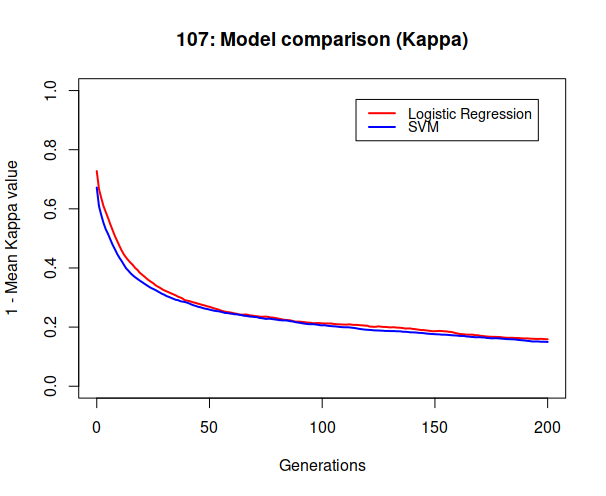
\includegraphics[width=0.45\textwidth]{gfx/FS_ModelComparison_Kappa_107.png}
				\end{varwidth}
			}
            \fbox{
				\begin{varwidth}{\textwidth}
					\centering
					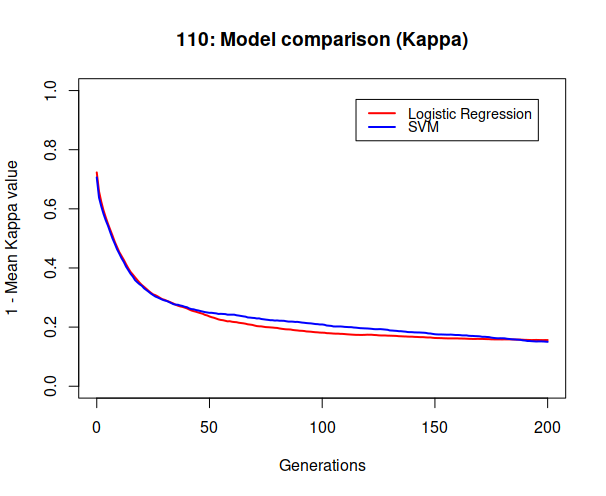
\includegraphics[width=0.45\textwidth]{gfx/FS_ModelComparison_Kappa_110.png}
				\end{varwidth}
			}

		\end{center}
		\caption[Kappa loss comparison with Logistic Regression and \acs{SVM}]{Comparison of Kappa loss evolution over time with Logistic Regression and \acs{SVM}.}\label{gfx:fs_models_kappa}

	\end{figure}

	From what we see, it is not clear which model to select. \acs{SVM} tends to converge more steadily, while the evolution of Logistic Regression tends to be steeper at the beginning. Neither one of them finish with clear advantage respect to the other, though.

	Perhaps the evolution of the cross-validation loss can help us assess their distinctive qualities. Figure \ref{gfx:fs_models_cv} contains the analogous plot. In it, we can observe how towards the right end of the curve the \acs{SVM}-driven experiment surpasses the other one in average performance. This is a sign that \acs{SVM}s could have an edge on Logistic Regressions for this dataset.

\newpage

	\begin{figure}[bth]

        \begin{center}

        	\setlength{\fboxrule}{0pt}
            \fbox{
				\begin{varwidth}{\textwidth}
					\centering
					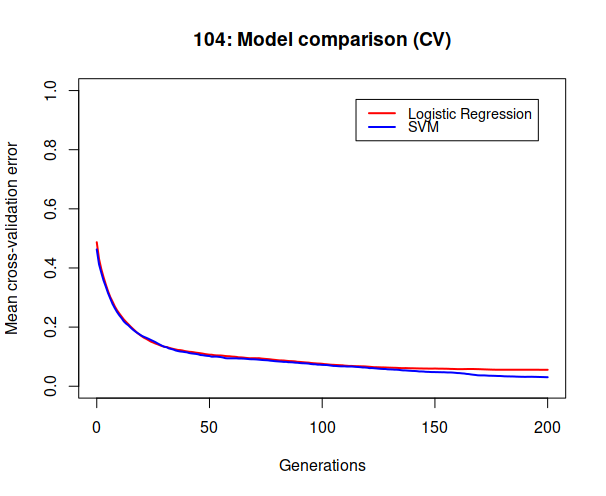
\includegraphics[width=0.45\textwidth]{gfx/FS_ModelComparison_CV_104.png}
				\end{varwidth}
			}
			\fbox{
				\begin{varwidth}{\textwidth}
					\centering
					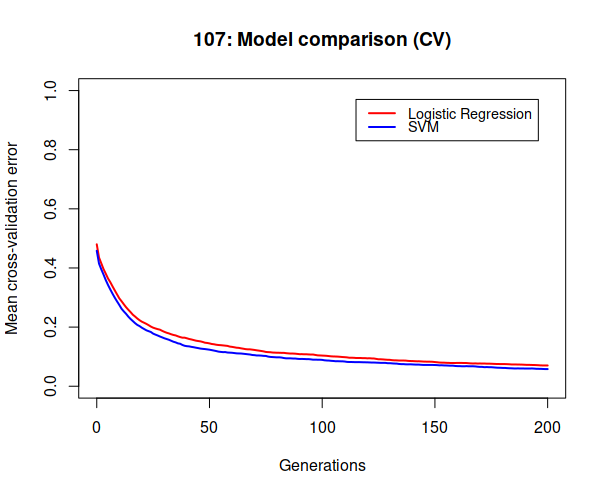
\includegraphics[width=0.45\textwidth]{gfx/FS_ModelComparison_CV_107.png}
				\end{varwidth}
			}
            \fbox{
				\begin{varwidth}{\textwidth}
					\centering
					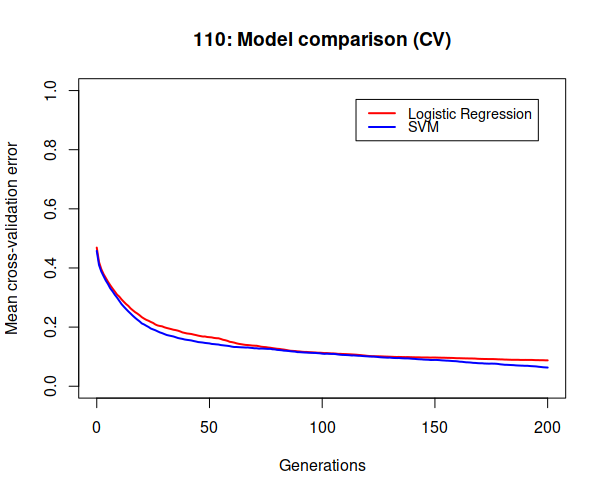
\includegraphics[width=0.45\textwidth]{gfx/FS_ModelComparison_CV_110.png}
				\end{varwidth}
			}

		\end{center}
		\caption[Cross-validation loss comparison with Logistic Regression and \acs{SVM}]{Comparison of cross-validation loss evolution over time with Logistic Regression and \acs{SVM}.}\label{gfx:fs_models_cv}

	\end{figure}

	Like we have already done twice, it is natural to record several experiments to confirm or dismiss what we have just seen. Making use of the best algorithm configurations found until now, Logistic Regression and \acs{SVM} (with $C = 0.1$) will be tested against each other by averaging their best Kappa loss from 15 runs. Table \ref{table:models_kappa} holds the numbers.

	\vspace{0.3cm}

	\begin{table}[h]

        \centering
        \setlength\arrayrulewidth{0.8pt}

        \begin{tabular}{| >{\centering\arraybackslash}m{0.5in} | >{\centering\arraybackslash}m{1.1in} | >{\centering\arraybackslash}m{1.1in} |}

            \hline
            \rowcolor{RoyalBlue}
            \textbf{Subject} & \textbf{SVM} & \textbf{LogReg} \\
            \hline
            \textbf{104} & $0.05127 \pm 0.0103$ & $0.05128 \pm 0.0067$ \\
            \hline
            \textbf{107} & $0.09546 \pm 0.0093$ & $0.12122 \pm 0.0126$ \\
            \hline
            \textbf{110} & $0.11796 \pm 0.0095$ & $0.13369 \pm 0.0083$ \\
            \hline

        \end{tabular}

        \caption{Comparison of average Kappa error values for the three subjects and the two models in question.}\label{table:models_kappa}

    \end{table}

    It is quite apparent that \acs{SVM}s provide yet another push in classification quality---it is also expected that cross-validation measures follow the same pattern, given that they triggered this comparison.

    In the next page we can find Table \ref{table:models_kruskal}, which contains the p-values for the Kruskal-Wallis test for statistically significant differences.

\newpage

     \begin{table}[h]

        \centering
        \setlength\arrayrulewidth{0.8pt}

        \begin{tabular}{| >{\centering\arraybackslash}m{0.9in} |  >{\centering\arraybackslash}m{0.9in} | >{\centering\arraybackslash}m{0.9in} |}

        	\hline
        	\rowcolor{RoyalBlue}
        	\multicolumn{3}{| >{\centering\arraybackslash}m{3.054in} |}{\textbf{Logistic Regression against SVM}} \\
            \hline
            \rowcolor{RoyalBlue}
            \textbf{104} & \textbf{107} & \textbf{110} \\
            \hline
            \textcolor{red}{$p = 0.917098$} & $p = 0.000025$ & $p = 0.000060$ \\
            \hline

        \end{tabular}

        \caption{Comparison of p-values for Logistic Regression and \acs{SVM} in all test subjects.}\label{table:models_kruskal}

    \end{table}

    Again, the test shows that there is often a relevant accuracy boost when using \acs{SVM} instead of Logistic Regression (in subject 104 we might have reached the full potential). Although we do not show them here, the cross-validation differences are noticeable too.

    It is also true that this change has taken a toll on the running time of the algorithm. Nevertheless---and following the same logic as when we increased population sizes and number of generations---, the improvements in quality of the solutions are crucial at this level. Since we can still run a couple dozen experiments a day (counting the three test subjects), we can safely sacrifice efficiency in favor of further gains.

	We have finally completed our review of feature selection enhancements. Although by now it should go without saying that feature selection is essential in our problem, Table \ref{table:feature_selection_comparison} puts our best results so far (in terms of Kappa loss) against classifiers using all 3600 features.

	\vspace{0.3cm}

    \begin{table}[h]

        \centering
        \setlength\arrayrulewidth{0.8pt}

        \begin{tabular}{| >{\centering\arraybackslash}m{0.7in} | >{\centering\arraybackslash}m{0.7in} | >{\centering\arraybackslash}m{0.7in} | >{\centering\arraybackslash}m{0.7in} | >{\centering\arraybackslash}m{0.7in} |}

			\hline
			\rowcolor{RoyalBlue}
			 & \multicolumn{2}{|c|}{\textbf{Feature selection}} & \multicolumn{2}{|c|}{\textbf{No feature selection}} \\
			\hline
            \rowcolor{RoyalBlue}
            \textbf{Subject} & \textbf{Log Reg} & \textbf{SVM} & \textbf{Log Reg} & \textbf{SVM} \\
            \hline
            \cellcolor{RoyalBlue}\textbf{104} & $0.042246$ & $0.033781$ & $0.279954$ & $0.305215$ \\
            \hline
            \cellcolor{RoyalBlue}\textbf{107} & $0.101059$ & $0.075823$ & $0.327885$ & $0.328009$ \\
            \hline
            \cellcolor{RoyalBlue}\textbf{110} & $0.117981$ & $0.101107$ & $0.404468$ & $0.404545$ \\
            \hline

        \end{tabular}

        \caption{Best Kappa loss scores of feature selection versus no feature selection.}\label{table:feature_selection_comparison}

    \end{table}

    Notice that we list both Logistic Regression and \acs{SVM} to introduce a bit more information: even though the former behaves better with no feature selection, it ultimately fails to equal the latter after both are optimized under the same conditions.

    These results constitute the baseline for the next two sections, which will be dedicated to the optimization of neural networks using the best features we have been able to obtain.

    Since the accuracy is already unexpectedly good, our efforts will be focused on discerning whether there is still room for improvement with the use of more advanced models (such as neural networks) or the remaining gap is just an intrinsic limitation of the data. We will also discuss the pros and cons of applying neural networks to this specific dataset.

\newpage

\section{Structure optimization}\label{sec:res_so}

	This section covers the first step of the proposed neural network optimization workflow: the search for a good structure.

	Before we start, it should be noted that, as opposed to feature selection---where time is not much of a concern---, from now on the experiments will be severely limited by the training process of neural networks. The decrease in population sizes and number of generations will be drastic (15 to 20 times less), but the running times will still be one order of magnitude higher if we cannot find any workarounds. This is one of the reasons why we have put so much effort into finding the right features.

	Having said that, let us begin by explaining the motivation for a two-step optimization. When we try to optimize several parameters at the same time, the combined search space is as big as the product of the sizes of the individual search spaces; this is often quite a lot, and the genetic algorithm has to work with accordingly bigger populations and evolution periods to make up for it. In an attempt to take away a part of this complexity, we can concede a (hopefully) small decrease in potential quality and try to optimize one (or a few) of those parameters in isolation.

	If we agree to the aforementioned logic, the first point in question is how to split the process in a way that the disruption to the overall optimization is minimized. Let us take a look at what parameters---hyperparameters--- we will be dealing with:

	\begin{itemize}

		\item
		Learning rate.

		\item
		Number of training epochs.

		\item
		Dropout rate.

		\item
		Structure (number of layers and units per layer).

	\end{itemize}

	It is possible to identify a pattern that divides them into two groups: the first three are discrete numbers that are adjusted once we have defined a model structure; the fourth is precisely that structure. Therefore, intuitively we may find a structure first and then use it to work out the best combination of the remaining hyperparameters.

	Assuming what we have just said, we need to determine how to optimize the structure while also looking for ways to speed up the process. For this, we will bring up the experimental results of last section. The high accuracies of linear models suggest that our neural networks should not be very complex, because if we couple that with our small training sets they will most likely suffer from overfitting.

\newpage

	Now, let us see how we can turn this in our favor. Suppose a population of 50 individuals and 20 generations, with the objective functions being again the Kappa loss and the 5-fold cross-validation. The amount of neural network trainings for each function is given by:

	\begin{itemize}

		\item
		Kappa: $50 \times 20 = 1000$ trainings.

		\item
		5-fold cross-validation: $5 \times 50 \times 20 = 5000$ trainings.

	\end{itemize}

	Which, summed up, yield a total of $6000$ trainings.

	Let us discuss the importance of each fitness measure in the process. The Kappa value uses the test set to give an estimate of how well the model will behave with unseen data. The cross-validation accuracy, however, assesses the generalization capability of the model (without using new data), which is directly tied to a low overfitting. Then, if we swap in a simplicity measure for the cross-validation function, we are still pushing in the same direction to an extent.

	The proposed simplicity measure is the sum of all the neurons of the given structure (note that the time it takes to compute it is negligible). This way, we can factor out $5000$ of the $6000$ evaluations or approximately $83\%$; in a more general statement, we are reducing the computational load of the fitness evaluation in a fraction very close to $\frac{k}{k+1}$, where $k$ is the number of cross-validation folds.

	Again, we have to keep in mind that this is only a fast alternative to improve the efficiency of this first optimization step---which is not the most important one. Also, it is derived from our previous results in this specific problem and, while there are experiments telling us that the speedup is worth the absence of cross-validation, further comparative testing would be required. Such testing is unfeasible in this work due to the large amounts of time needed for cross-validation.

	However, despite not being able to statistically analyze their differences, a single visual comparison contains a lot of information. Figure \ref{gfx:cv_vs_simplicity} shows the evolution of a sample Kappa-CV run against a sample Kappa-Simplicity run; the first one had 30 individuals and 20 generations, while the second one had 50 individuals (thus taking advantage of the speedup to have a bigger population).

	The first thing we notice is that the algorithm does not produce as significant a quality boost as in feature selection. Instead, it starts at an already decent point and tries to make improvements by evaluating new structures. Because it is only one of several hyperparameters to tune, it is not unusual to observe little average performance gains in both alternatives. Still, if we take a look at peak accuracy, Table \ref{table:best_cv_vs_simplicity} shows that these preliminary results are promising.

	Another aspect we can analyze is the time they take to reach their best average. Without making too many assumptions, it seems that the simplicity measure makes that time shorter, while with cross-validation we still find improvements later on. This suggests that we could add more individuals in exchange for less generations.

\newpage

	\begin{figure}[bth]

        \begin{center}

        	\setlength{\fboxrule}{0pt}
            \fbox{
				\begin{varwidth}{\textwidth}
					\centering
					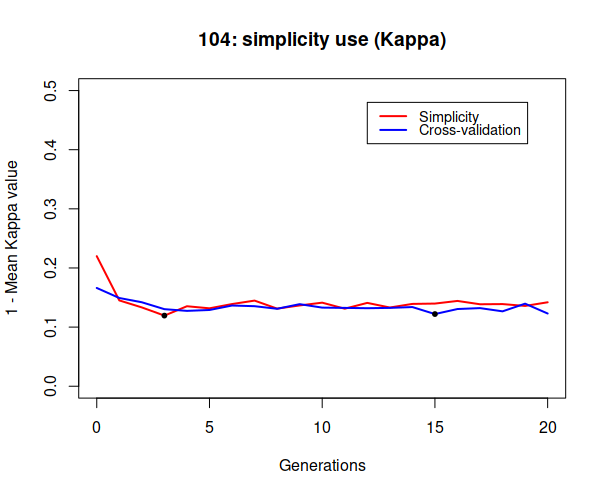
\includegraphics[width=0.45\textwidth]{gfx/SO_Simplicity_Kappa_104.png}
				\end{varwidth}
			}
			\fbox{
				\begin{varwidth}{\textwidth}
					\centering
					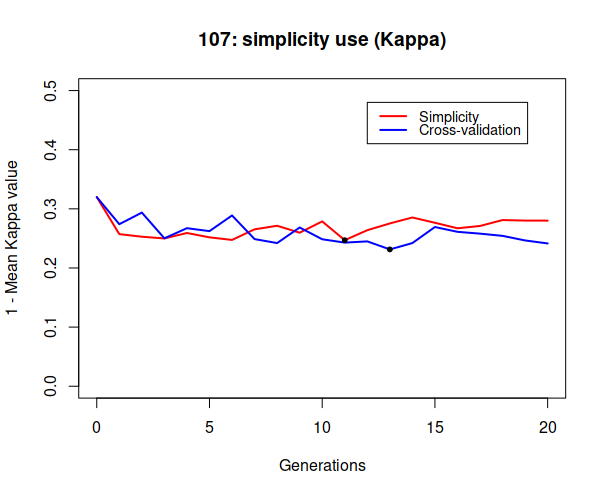
\includegraphics[width=0.45\textwidth]{gfx/SO_Simplicity_Kappa_107.png}
				\end{varwidth}
			}
            \fbox{
				\begin{varwidth}{\textwidth}
					\centering
					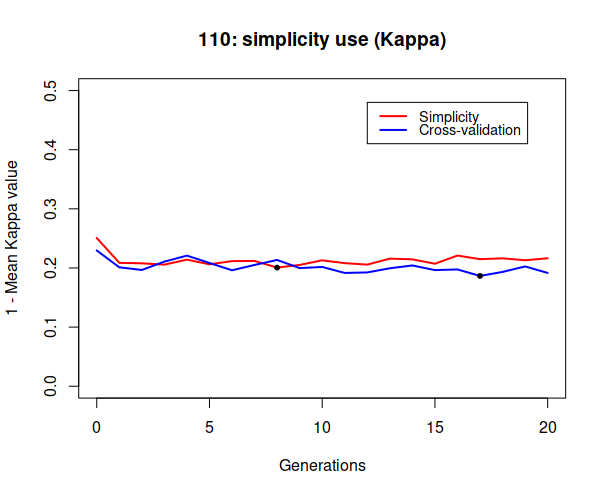
\includegraphics[width=0.45\textwidth]{gfx/SO_Simplicity_Kappa_110.png}
				\end{varwidth}
			}

		\end{center}
		\caption[Evolution comparison with cross-validation and simplicity]{Comparison of mean Kappa loss evolution for both metrics. Notice that the vertical axis now has the range $[0,0.5]$, as opposed to the previous $[0,1]$ used in feature selection.}\label{gfx:cv_vs_simplicity}

	\end{figure}

	\begin{table}[h]

        \centering
        \setlength\arrayrulewidth{0.8pt}

        \begin{tabular}{| >{\centering\arraybackslash}m{0.5in} | >{\centering\arraybackslash}m{1.2in} | >{\centering\arraybackslash}m{1.2in} |}

            \hline
            \rowcolor{RoyalBlue}
            \textbf{Subject} & \textbf{Cross-validation} & \textbf{Simplicity} \\
            \hline
            \textbf{104} & $0.09289$ & $0.08456$ \\
            \hline
            \textbf{107} & $0.16840$ & $0.19395$ \\
            \hline
            \textbf{110} & $0.15169$ & $0.17690$ \\
            \hline

        \end{tabular}

        \caption[Best Kappa values using cross-validation and simplicity]{Comparison of top Kappa error values for both metrics.}\label{table:best_cv_vs_simplicity}

    \end{table}

    As we can see in the table, the run employing simplicity trails behind a bit in peak performance but it manages to snatch the first place for subject 104. Knowing that it took much less time (1000 evaluations versus 3600), we can say that the tradeoff is more than fair.

    After this intuitive exploration, further comparative testing would be required. Such testing is not feasible because cross-validation is computationally too heavy. However, at 30-40 minutes per subject, we can afford to average a number of simplicity-driven experiments. 

    Let us define the parameters first: we will use 60 individuals and 15 generations; the hidden layers will be limited to 4, which will produce a first population of rather complex models to be reduced by simplicity; the crossover (midpoint) and mutation (single layer and uniform scaling) probabilities will be $0.1$ and $0.9$; the neural network fitting epochs will be fixed to 25; finally, we will repeat the combination Kappa-Simplicity.

\newpage

    Table \ref{table:average_peak_kappa_simplicity} shows the mean and peak Kappa loss for the three test subjects:

    \vspace{0.3cm}

    \begin{table}[h]

        \centering
        \setlength\arrayrulewidth{0.8pt}

        \begin{tabular}{| >{\centering\arraybackslash}m{0.7in} | >{\centering\arraybackslash}m{1.1in} | >{\centering\arraybackslash}m{1.1in} |}

			\hline
			\rowcolor{RoyalBlue}
			 & \textbf{Average} & \textbf{Best} \\
            \hline
            \cellcolor{RoyalBlue}\textbf{104} & $0.09037 \pm 0.0089$ & $0.07598$ \\
            \hline
            \cellcolor{RoyalBlue}\textbf{107} & $0.21734 \pm 0.0328$ & $0.14319$ \\
            \hline
            \cellcolor{RoyalBlue}\textbf{110} & $0.20895 \pm 0.0147$ & $0.18543$ \\
            \hline

        \end{tabular}

        \caption{Average and best Kappa loss scores of ten simplicity-driven test runs.}\label{table:average_peak_kappa_simplicity}

    \end{table}

    Figure \ref{gfx:best_simplicity_evolution} supports the hypothesis that the pair Kappa-Simplicity is able to improve from an initial, unoptimized population. It is manifest that the average Kappa loss again converges soon, but we cannot risk losing an eventual peak in performance by diminishing the generation count excessively---early average convergence does not prevent top individuals from appearing.

    \vspace{0.2cm}

	\begin{figure}[bth]

        \myfloatalign
        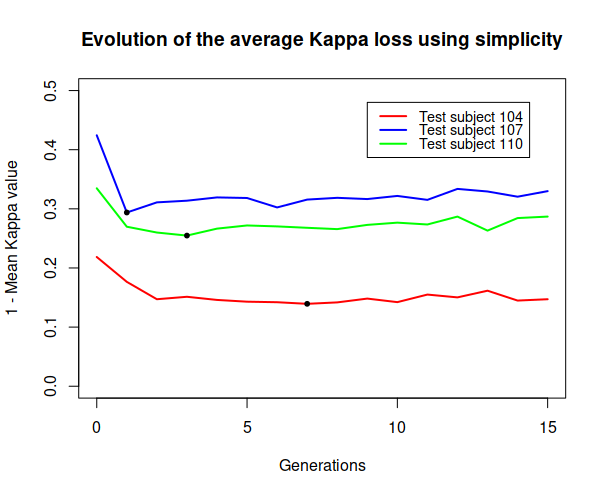
\includegraphics[width=0.9\textwidth]{gfx/SO_SimplicityEvolution.png}
        \caption{Evolution of the three experiments that produced the best peak accuracies.}\label{gfx:best_simplicity_evolution}

    \end{figure}

    In this section we have applied our previous knowledge to obtain neural network structures in short timespans. With them as a foundation, \textit{learning optimization}---as we will call the last step---will be crucial in deciding if the whole process is able to produce competitive enough models.

\section{Learning optimization}\label{sec:res_lo}

	This arduous search process finds its conclusion in the optimization of the hyperparameters we left aside in last section: learning rate, dropout rate and number of training epochs. Let us begin by reviewing them:

	\begin{itemize}

		\item
		Learning rate: when samples are processed through a neural network during training, we can trace what made the network's output differ from the true label; additionally, the error can be quantified from the weights of the connections. The learning rate is the fraction of the error used to correct those weights. Therefore, its values are in the range $(0,1]$.

		\item
		Dropout rate: dropout is a technique introduced recently \cite{srivastava2014dropout} that consists in disabling a certain number of randomly chosen units during each training step. This serves as a regularization method, because the final model is like an ensemble of weaker neural networks that represent the sets of units that remained active at each step. It can range between $0$ and $1$, but the authors recommend trying from $0.2$ to $0.5$.

		\item
		Number of epochs: an epoch is an iteration over the entire dataset, meaning that in one epoch there can be multiple weight updates depending on how many samples are used to calculate the error. It ranges from $1$ to as many as needed.

	\end{itemize}
